\chapter{Introducción a la terminal}
\section{Preámbulo}
Saber utilizar la terminal es una habilidad clave para el uso de Linux. Cualquier informático/a que sea capaz de utilizar la terminal de forma eficiente es capaz incluso de sobrepasar la eficiencia de las interfaces gráficas.

A pesar de que parezca lo contrario, aprender a usar la terminal no es una cuestión de memorización, sino de compresión. Es importante conocer cómo funciona Linux como sistema operativo.

Una habilidad muy importante para aprender a usar la terminal (y para cualquier ámbito de la informática realmente) es saber buscar información. Esto significa saber buscar en foros, filtrar información, y saber cómo formular tus dudas en el buscador.

Para terminar, cabe recalcar la importancia de la práctica. La práctica es la clave para dominar la terminal. Usarla lo máximo posible en tu día a día hará que poco a poco te vayas acostumbrando a su funcionamiento. La mayoría de tus habilidades usando la terminal se conseguirán de forma pasiva, haciendo otras actividades o proyectos en ella.

Una forma muy buena de practicar la terminal es simplemente pasarse a Linux. Para empezar puedes configurar tu máquina para que sea dual boot (sistema operativo dual, en este caso tu sistema operativo habitual + Linux), así puedes probar Linux sin necesariamente eliminar tu SO original.

\section{Introducción}
Una terminal es una Interfaz de Línea de Comandos (CLI, Command Line Interface en inglés). Es la alternativa a las conocidas GUIs (Guided User Interface, las interfaces que utilizamos día a día). Una CLI es una interfaz notablemente más sencilla que una GUI, ya que solo contiene texto.

La terminal nos da un control más profundo y preciso de nuestro sistema. Mediante comandos, podemos comunicarnos con nuestra máquina para realizar tareas más complejas. Sin embargo, una terminal no es más que un intermediario entre el usuario/a y un shell.

Un shell, esencialmente, es un intérprete de comandos. Cuando escribimos en una terminal, lo que realmente estamos haciendo es comunicarnos con un shell. Es el shell quien se encarga de realizar las tareas. Uno de los shells más utilizados en Linux por diferencia es bash (Bourne Again SHell), creado por GNU.

Un comando puede considerarse una "orden" dictada por el usuario. Sigue una estructura fija (pero que puede cambiar entre comandos diferentes) que puede contener argumentos. Un argumento es información adicional que le proporcionamos al comando. Algunos argumentos pueden ser obligatorios (es decir, que tenemos que especificarlos si queremos ejecutar un comando), mientras que otros son opcionales. Veamos un ejemplo de comando:

\begin{tcolorbox-code}
\begin{lstlisting}
$ echo "hello world"
hello world
\end{lstlisting}
\end{tcolorbox-code}

echo es un comando en bash que te devuelve el o los argumentos que le proporcionas. En este caso, le hemos proporcionado un argumento en forma de string. Por tanto, lo que nos devuelve va a ser precisamente "hello world".


Además de los argumentos, existe otro campo principal que puede tener un comando. A este se le llama opción. Una opción es otro tipo de argumento, normalmente iniciado con uno o dos guiones (-). Un comando puede tener diferentes funcionalidades. Estas funcionalidades normalmente se suelen especificar utilizando una opción. Veamos un ejemplo:

\begin{tcolorbox-code}
\begin{lstlisting}
$ shutdown
\end{lstlisting}
\end{tcolorbox-code}

shutdown es un comando que por defecto apaga tu equipo tras una cuenta atrás de 60 segundos si no le proporcionas ningún argumento más. Sin embargo, una de las opciones que tiene este comando es -r (reboot).

\begin{tcolorbox-code}
\begin{lstlisting}
$ shutdown -r
\end{lstlisting}
\end{tcolorbox-code}

Si le proporcionas esta opción, en vez de apagarse, el sistema se reiniciará en 60 segundos.

Cada comando tiene diferentes argumentos y opciones, por eso es importante consultar información sobre éstos si no los hemos usado antes. Más sobre esto más tarde.

Con estos conocimientos básicos, ya podemos empezar a utilizar la terminal.

\section{Entrando a la terminal}
La forma de entrar a tu terminal depende de tu Desktop Environment. Por ejemplo, si estás en Ubuntu con GNOME (el DE por defecto de la distribución), basta con acceder al menú y abrir la consola. En muchos Desktop Environments también puedes abrir una terminal con la combinación de teclas ctrl + alt + t.

Al abrir la terminal nos encontraremos con una ventana similar a esta:
\begin{figure}[H]
    \centering
    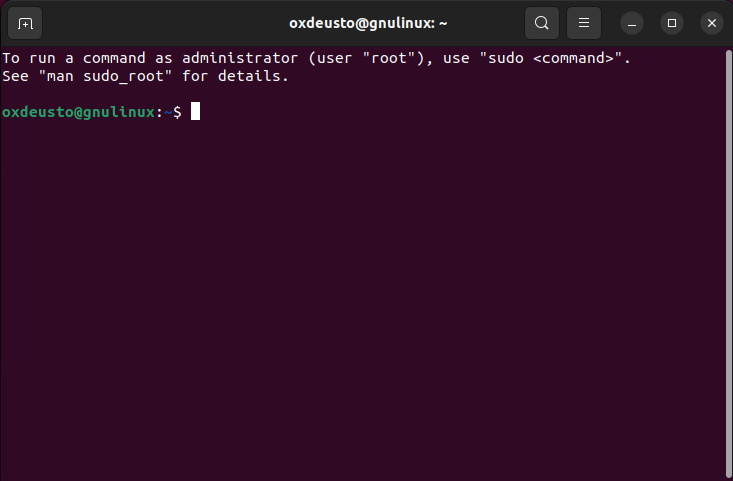
\includegraphics[width=0.80\linewidth]{resources/images/terminal_abrir.png}
    \caption{Aspecto de la terminal al abrirla}
\end{figure}

Vamos a fijarnos en el texto:

\begin{tcolorbox-code}
\begin{lstlisting}
oxdecode@gnulinux:~$
\end{lstlisting}
\end{tcolorbox-code}

A este texto se le llama shell prompt. ¿Pero qué significa? Vamos a verlo por partes:

\begin{itemize}
    \item Nuestro nombre de usuario se encuentra a la izquierda del carácter @ (que hace de separador). En este caso es "oxdecode".
    \item Después del @ está nuestro hostname (el nombre de nuestro ordenador), también configurado por nosotros al instalar el sistema. En este caso es "gnulinux".
    \item El carácter \~{} es un carácter especial. Siempre que lo veas en el shell prompt significa que te encuentras en tu directorio de usuario en /home. En este caso, la dirección absoluta sería /home/oxdecode Además, es la dirección por defecto en que se abre la terminal. Si en el directorio de usuario hubiera otro directorio llamado "fotos", y se abriera la terminal ahí, el shell prompt sería así:

    \begin{tcolorbox-code}
\begin{lstlisting}
    oxdecode@gnulinux:~/fotos$
\end{lstlisting}
\end{tcolorbox-code}

    \item El carácter del dólar (\$) al final del prompt no es más que un indicador que muestra que puedes escribir comandos a nivel de usuario. Si en vez de salir un \$ saldría un \#, significa que tienes permisos de root.
\end{itemize}

\section{Direcciones}
Ahora que has visto direcciones en el shell prompt, es hora de hablar sobre cómo funcionan. Como se mencionó en el Tema 2, la forma en la que se ordenan los ficheros en un sistema operativo de Linux es jerárquica. Todos los directorios y ficheros parten de un solo sitio, root. Esta es su dirección:

\begin{tcolorbox-code}
\begin{lstlisting}
/
\end{lstlisting}
\end{tcolorbox-code}

En root se encuentran todos los directorios del SO, como /home, /etc, /tmp... El directorio de nuestro usuario se encuentra en /home, donde están todos los directorios de usuarios. Si tu nombre de usuario es "oxdecode", la dirección del directorio será la siguiente:

\begin{tcolorbox-code}
\begin{lstlisting}
/home/oxdecode/
\end{lstlisting}
\end{tcolorbox-code}

El direccionamiento es la forma que tenemos de localizar archivos, ya sea para referenciarlos en un programa o para abrirlos nosotros mismos. Hay dos tipos de direccionamiento:

\begin{itemize}
    \item \textbf{Direccionamiento absoluto}: Cuando referencias la dirección del fichero desde root (/). La ventaja de utilizar el direccionamiento absoluto es que la dirección va a ser válida independientemente del directorio en el que te encuentres, porque inicias el direccionamiento desde root. Un ejemplo de direccionamiento absoluto es precisamente el ejemplo de dirección previo:
    \begin{tcolorbox-code}
\begin{lstlisting}
/home/oxdecode/
\end{lstlisting}
\end{tcolorbox-code}
    \item \textbf{Direccionamiento relativo}: Cuando referencias la dirección del fichero desde el directorio en el que estás trabajando. La ventaja de este tipo de direccionamiento es que puede ser muy útil en programas de código. Si quieres programar una aplicación que necesite referenciar un archivo en el mismo directorio en el que se ejecuta la aplicación, es más conveniente utilizar direccionamiento relativo, ya que tú, como programador/a, no tienes por qué conocer la estructura de archivos de un ordenador que no es tuyo. Fíjate en esta estructura de archivos:
\end{itemize}

\begin{figure}[H]
    \centering
    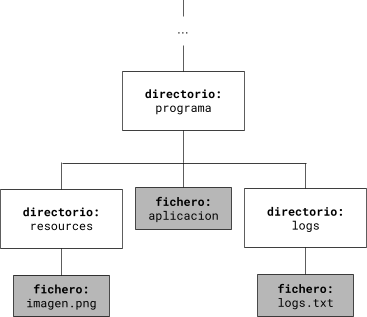
\includegraphics[width=0.80\linewidth]{resources/images/estructura-archivos-1.png}
    \caption{Estructura de archivos de ejemplo}
\end{figure}

Tenemos un directorio llamado "programa", con otros dos directorios dentro, "resources" y "logs". Los tres puntos indican que no sabemos dónde está almacenado "programa", pero no nos importa porque podemos utilizar el direccionamiento relativo para referenciar los ficheros que sí sabemos dónde están, "imagen.png" (en programa/resources), "logs.txt" (en programa/logs) y "aplicación" (que es un fichero ejecutable en programa).

Pongamos que el programa aplicación necesita utilizar el fichero "imagen.png". Para ello, podemos poner en el código la ruta relativa de la imagen. Como el fichero está en programa, la ruta relativa de la imagen es esta:

\begin{tcolorbox-code}
\begin{lstlisting}
resources/imagen.png\begin{figure}
\end{lstlisting}
\end{tcolorbox-code}

Pon atención a que no escribimos una barra al principio de la dirección, porque de escribirla estaríamos accediendo al fichero desde root, de forma absoluta, algo indeseado para este ejemplo, ya que no encontraría el fichero. Como resources está directamente dentro de "programa", podemos referenciarlo directamente, sin poner nada previamente. Es por esto que el direccionamiento relativo es tan útil.

Vamos ahora con un ejemplo un poco más raro: por lo que sea, ahora el programa se encuentra en la carpeta programa/resources, y queremos acceder a logs.txt. La estructura de archivos es esta:

\begin{figure}[H]
    \centering
    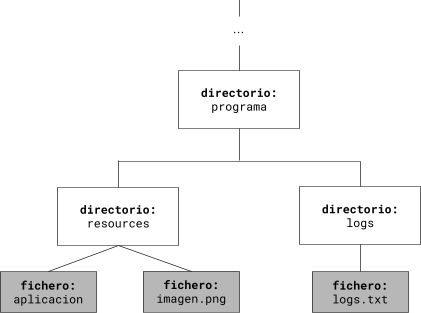
\includegraphics[width=0.80\linewidth]{resources/images/estructura_ficheros_2.png}
    \caption{Otra estructura de archivos.}
\end{figure}

Aquí acceder a logs.txt es un poco más complicado, porque tenemos que ir hacia atrás para acceder al directorio de programa/logs. La forma de acceder a logs.txt desde resources sería la siguiente:

\begin{tcolorbox-code}
\begin{lstlisting}
../logs/logs.txt
\end{lstlisting}
\end{tcolorbox-code}

Al incluir dos puntos en la dirección estamos representando que queremos dar "un paso para atrás" en la jerarquía de directorios. Al usarlos, en este caso nos iríamos al directorio "programa", donde podemos acceder a logs y posteriormente a logs.txt.

Cabe destacar que el direccionamiento relativo no solo se usa en código de programas, lo podemos utilizar también en comandos de terminal, si así lo necesitamos. Veremos cómo en el siguiente apartado.

\section{Navegando entre directorios}
Como hemos aprendido en el apartado anterior, las direcciones son esenciales para trabajar en la terminal. Hemos visto también cómo la terminal puede estar en una dirección u otra, y cómo afecta eso a nuestras tareas. Una de las cosas que más se suele hacer es desplazarse alrededor de tu sistema de archivos. Para ello se utiliza el comando cd.

cd (o change directory) es un comando que, como su propio nombre indica, nos permite movernos entre directorios. El uso es muy simple:

\begin{tcolorbox-code}
\begin{lstlisting}
$ cd <dirección del directorio>
\end{lstlisting}
\end{tcolorbox-code}

Como ejemplo vamos a imaginarnos que estamos en el directorio /var y que queremos movernos al directorio de nuestro usuario. Una forma de hacerlo sería la siguiente.

\begin{tcolorbox-code}
\begin{lstlisting}
$ cd /home/oxdecode
\end{lstlisting}
\end{tcolorbox-code}

En este caso estamos utilizando la dirección absoluta de nuestro directorio para movernos a él. Sin embargo, hay otra forma más rápida de acceder a este directorio. Como hemos mencionado anteriormente, el carácter ~ se suele asociar con nuestro directorio de usuario. Observa:

\begin{tcolorbox-code}
\begin{lstlisting}
$ cd ~
\end{lstlisting}
\end{tcolorbox-code}

Este comando es otra forma igual de válida que la otra para acceder a tu directorio de usuario. De hecho, los dos comandos son equivalentes. Además, puedes usar el mismo carácter para acceder a otros directorios en el directorio de usuario. Considerando que creamos el directorio "fotos" dentro del directorio y que seguimos en /var (aunque este ejemplo funciona en cualquier directorio ya que es direccionamiento absoluto)...

\begin{tcolorbox-code}
\begin{lstlisting}
$ cd ~/fotos 
\end{lstlisting}
\end{tcolorbox-code}

Este comando nos movería a "fotos". Y ya para terminar, podemos volver a nuestro directorio de usuario de forma relativa.

\begin{tcolorbox-code}
\begin{lstlisting}
$ cd ..
\end{lstlisting}
\end{tcolorbox-code}

Ten en cuenta que el doble punto se puede usar más de una vez para moverse más hacia atrás. Desde ~, poniendo el doble punto dos veces, llegaríamos a root (el primer doble punto nos llevaría a /home y el segundo a /):

\begin{tcolorbox-code}
\begin{lstlisting}
$ ../..
\end{lstlisting}
\end{tcolorbox-code}

Cabe mencionar la existencia del comando pwd (Print Working Directory), un comando que nos imprime la dirección absoluta del directorio en el que nos encontramos. Si me encuentro en ~/fotos y ejecuto el comando nos devolvería esto:

\begin{tcolorbox-code}
\begin{lstlisting}
$ pwd
/home/oxdecode/fotos
\end{lstlisting}
\end{tcolorbox-code}

Con toda esta información, ya sabemos lo básico sobre la terminal y cómo navegar en ella. Es momento de aprender todo lo demás. En el próximo tema empezaremos con bash, aprendiendo unos comandos variados que nos ayudarán a adaptarnos poco a poco a usar la terminal de forma cotidiana.
